\chapter{Utilisation par un terminal}
\label{chap:useterm}

\renewcommand{\labelitemi}{$\bullet$} %changer les puces pour cette page

LoCD peut être utilisé uniquement en ligne de commande. Cette partie demandes des connaissances pré requises sur les commandes unix. En effet seul les fonctionalités de l'outil seront explicitées. La mecanisme des options est similaire à toute autres commandes unix. Pour plus de d'information sur les système \gls{unix}, nous recommandons l'ouvrage suivant : \cite{linux}.

%%%%%%%%%%%%%%%%%%%%%%%%%%%%%%%%%%%%%%%%%%%%%%%%%%%%%%%%%%%%%%%%%%%%%%%%%

\section{Utilisation basique}
\label{sec:usebas}
La simple commande suivante générera un pdf avec d'un histogrammes avec les paramètres par défaut : % rajouter ref!!!!!!!!!!!!!!!!!!!!!!!!!!!!!!!
\begin{verbatim}LoCD inputfile.txt\end{verbatim}Les choix du type de diagramme est possible grâce à l'option \verb+-d+ (ou \verb+--diagramme+) suivit de : 
\begin{itemize}
\item
\verb+circulaire+ pour un diagramme circulaire.
\item
\verb+histogramme+ pour un histogramme.
\item
\verb+nuage+ pour un diagramme en nuage de points.
\end{itemize}

%%%%%%%%%%%%%%%%%%%%%%%%%%%%%%%%%%%%%%%%%%%%%%%%%%%%%%%%%%%%%%%%%%%%%%%%%

\section{Gestion des méta données}
Une option pour chacune des méta données disponible (cf : ~\ref{chap:fichDonnees}) est définie :
\begin{itemize}
\item
\verb+-t+ ou \verb+--title+ pour afficher le \gls{titre}. 
\item
\verb+-s+ ou \verb+--subtitle+ pour afficher le \gls{sous titre}.
\item
\verb+-n+ ou \verb+--note+ pour afficher la \gls{note}.
\end{itemize}
Si une de ces options est renseignée, il est possible de rajouter une valeur pour le paramêtre concerné. Par exemple : 
\begin{verbatim}
  LoCD --title "Mon titre de diagramme" --subtitle "le sous" titre"
\end{verbatim} 
Dans le cas où l'une de ces options serait rajoutée ; et que aucune valeur ne lui est attribuée (en ligne de commande ou dans le fichier d'entrée) ; un avertissement apparaîtra à l'execution. Le diagramme n'aura pas de sous titre.
  \begin{figure}[htbp]
    \centering
    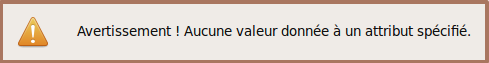
\includegraphics[scale=0.90]{img/aattributs}
    \caption{Avertissement : option manquante}
    \label{fig:optmissing}
  \end{figure}  

%%%%%%%%%%%%%%%%%%%%%%%%%%%%%%%%%%%%%%%%%%%%%%%%%%%%%%%%%%%%%%%%%%%%%%%%%
\section{Mise en forme reglages divers}
Le diagramme obtenu dans le cas d'une utilisation basique (~\ref{sec:usebas}) est stocké dans le dossier courant sous le nom de \verb+new_file.pdf+ et a les caractéristiques graphiques suivantes illustrée dans la figure :  ~\ref{fig:dbatons}.\\ Le changement du nom de ficher de sortie peut être modifier en rajoutant l'option \verb+-f outfilename+ ou dans sa version longue \verb+--filename+. 
\subsection{Couleurs}
\label{subsec:couleurs}
L'option \verb+-c+ (ou \verb+--couleur+) permet d'éditer la couleur de chaque données. Dans cette version LoCD propose une palette de 6 couleurs :
\begin{itemize}
\item
  orange
\item
  rouge
\item
  vert
\item
  bleu
\item
  bleu ciel
\item
  violet
\end{itemize}
Deux méthodes sont possibles :
\begin{enumerate}
\item
  Faire suivre l'option d'un nom de couleur (listées ci-dessus). Le diagramme aura alors cette unique couleur.
\item
  Faire suivre l'option du nom de la donnée puis d'un «couple» nom\_donnee:couleur séparé par le caractère \verb+:+. Une ou toutes les données peuvent être ainsi précisées. Dans tout autre cas, la couleur par défaut sera appliquée.
\end{enumerate}   
\subsection{Mise en page}
\label{subsec:misepage}
Dans la configuration par défaut. Le diagramme est centrée dans une page de format A4 («au centre»). Le titre et le sous titre sont placés au dessus du diagramme (au nord»). La note elle, est placée à droite de des titres («nord est»). La figure \ref{fig:dnuages} est l'illustration de cette mise en page par défaut. 
  \paragraph{Changement de type de papier :}
  \label{par:chgtpap}
  Lors de l'execution il est possible d'indiquer le type de papier à l'aide de l'option \verb+-f+ (ou \verb+ --feuilleformat+) et renseigner le format :
  \begin{itemize}
  \item
    A4
  \item
    A3
  \item
    Legal US
  \item
    B5
  \end{itemize} 
  \paragraph{Positionement des composant :}
  \label{par:poscompo}
  Pour changer cette dernière, il est possible de procéder d'une manière analogue à la configuration des couleurs. Ainsi l'option \verb+-p+ (ou \verb+--position+) suivi d'un des mots clefs, cités ci-après, permettent de positioner globalement le diagramme dans la page : 
  \begin{itemize}
  \item
    nord
  \item
    sud
  \item
    ouest
  \item
    est
  \end{itemize}
  Les conbinaisons cohérentes de deux orientations est possible en les collant. Exemple : \verb+-p nordest+. Pour préciser un placement uniquement à un composant on utilise à nouveau le caractère \verb+:+ séparant le nom du composant de son placement : \verb+--position note:sud+. 
  \footnote{En cas de conflits, LoCD placera «au mieu» les composant dans la page.}

  \subsection{Exemple :}
  \label{subsec:excom}
  Pour synthétiser ce chapitre consacré à l'utlilisation de LoCD en ligne de commande, voici un cas d'utilisation qui avec fichier de données approprié aboutira au diagramme de la figure ~\ref{fig:dnuages} : 

  \begin{figure}[htbp]
    \centering
    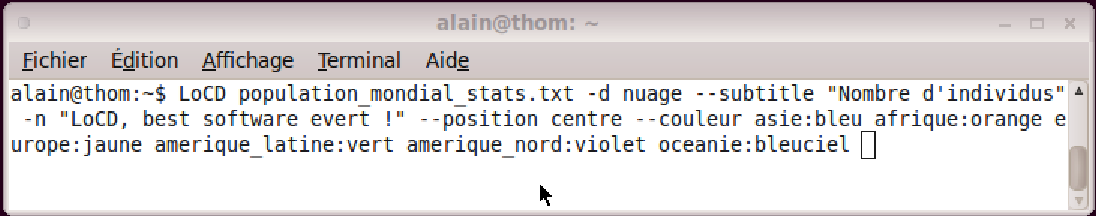
\includegraphics[scale=0.40]{img/ecommandes}
    \caption{Exemple d'utilisation de LoCD en ligne de commandes.}
    \label{fig:ecommandes}
  \end{figure}  
